\protect\hyperlink{main-nav}{≡} \protect\hyperlink{close-nav}{×}

\hypertarget{section-1.6-polynomials-and-rational-functions}{%
\section{Section 1.6: Polynomials and Rational
Functions}\label{section-1.6-polynomials-and-rational-functions}}

\hypertarget{polynomial-functions}{%
\subsection{Polynomial Functions}\label{polynomial-functions}}

\hypertarget{terminology-of-polynomial-functions}{%
\paragraph{Terminology of Polynomial
Functions}\label{terminology-of-polynomial-functions}}

A polynomial is a function that can be written as \textbackslash{}{[}
f(x)=a\_0+a\_1 x+a\_2 x\^{}2+\textbackslash{}dots+a\_n x\^{}n
\textbackslash{}{]}

Each of the \textbackslash{}(a\_i\textbackslash{}) constants are called
\textbf{coefficients} and can be positive, negative, or zero, and be
whole numbers, decimals, or fractions.

A \textbf{term} of the polynomial is any one piece of the sum, that is
any \textbackslash{}( a\_i x\^{}i \textbackslash{}). Each individual
term is a transformed power function.

The \textbf{degree} of the polynomial is the highest power of the
variable that occurs in the polynomial.

The \textbf{leading term} is the term containing the highest power of
the variable: the term with the highest degree.

The \textbf{leading coefficient} is the coefficient of the leading term.

Because of the definition of the ``leading'' term we often rearrange
polynomials so that the powers are descending: \textbackslash{}{[}
f(x)=a\_n x\^{}n+a\_\{n-1\}x\^{}\{n-1\}\textbackslash{}dots a\_2
x\^{}2+a\_1 x+a\_0 \textbackslash{}{]}

\hypertarget{example-1}{%
\paragraph{Example 1}\label{example-1}}

Identify the degree, leading term, and leading coefficient of the
polynomial \textbackslash{}( f(x)=3+2x\^{}2-4x\^{}3 \textbackslash{})

The degree is 3, the highest power on
\textbackslash{}(x\textbackslash{}). The leading term is the term
containing that power, \textbackslash{}( -4x\^{}3 \textbackslash{}). The
leading coefficient is the coefficient of that term, -4.

\hypertarget{short-run-behavior-intercepts}{%
\subsubsection{Short Run Behavior:
Intercepts}\label{short-run-behavior-intercepts}}

As with any function, the vertical intercept can be found by evaluating
the function at an input of zero. Since this is evaluation, it is
relatively easy to do it for a polynomial of any degree. To find
horizontal intercepts, we need to solve for when the output will be
zero. For general polynomials, this can be a challenging prospect.
Consequently, we will limit ourselves to three cases:

\begin{enumerate}
\tightlist
\item
  The polynomial can be factored using known methods: greatest common
  factor and trinomial factoring.
\item
  The polynomial is given in factored form.
\item
  Technology is used to determine the intercepts.
\end{enumerate}

\hypertarget{example-2}{%
\paragraph{Example 2}\label{example-2}}

Find the horizontal intercepts of \textbackslash{}(
f(x)=x\^{}6-3x\^{}4+2x\^{}2 \textbackslash{}).

We can attempt to factor this polynomial to find solutions for
\textbackslash{}(f(x) = 0\textbackslash{}):

\begin{longtable}[]{@{}ll@{}}
\toprule
\endhead
\textbackslash{}(x\^{}6-3x\^{}4+2x\^{}2=0\textbackslash{})
&\tabularnewline
\textbackslash{}(x\^{}2(x\^{}4-3x\^{}2+2)=0\textbackslash{}) & Factoring
out the greatest common factor\tabularnewline
\textbackslash{}(x\^{}2(x\^{}2-1)(x\^{}2-2)=0\textbackslash{}) &
Factoring the inside as a quadratic in
\textbackslash{}(x\^{}2\textbackslash{})\tabularnewline
\bottomrule
\end{longtable}

Then break apart to find solutions:

\begin{longtable}[]{@{}lllll@{}}
\toprule
\endhead
\textbackslash{}( x\^{}2=0 \textbackslash{}) & & \textbackslash{}(
x\^{}2-1=0 \textbackslash{}) & & \textbackslash{}( x\^{}2-2=0
\textbackslash{})\tabularnewline
\textbackslash{}(x=0\textbackslash{}) & &
\textbackslash{}(x\^{}2=1\textbackslash{}) & & \textbackslash{}(
x\^{}2=2 \textbackslash{})\tabularnewline
\textbackslash{}(x=0\textbackslash{}) & or & \textbackslash{}(
x=\textbackslash{}pm 1 \textbackslash{}) & or & \textbackslash{}(
x=\textbackslash{}pm\textbackslash{}sqrt\{2\}
\textbackslash{})\tabularnewline
\bottomrule
\end{longtable}

This gives us five horizontal intercepts.

\hypertarget{example-3}{%
\paragraph{Example 3}\label{example-3}}

Find the horizontal intercepts of \textbackslash{}(
h(t)=t\^{}3+4t\^{}2+t-6 \textbackslash{})

Since this polynomial is not in factored form, has no common factors,
and does not appear to be factorable using techniques we know, we can
turn to technology to find the intercepts.

Graphing this function, it appears there are horizontal intercepts at
\textbackslash{}(t =\textbackslash{}) -3, -2, and 1.

\begin{figure}
\centering
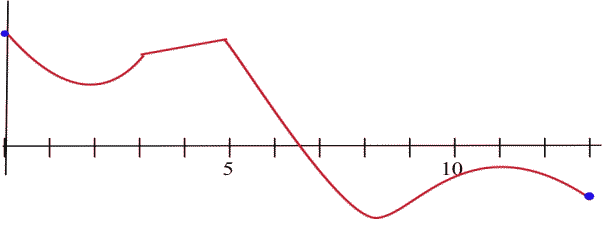
\includegraphics{images/image067.png}
\caption{}
\end{figure}

We could check these are correct by plugging in these values for
\textbackslash{}(t\textbackslash{}) and verifying that \textbackslash{}(
h(-3)=h(-2)=h(1)=0 \textbackslash{}).

\hypertarget{solving-polynomial-inequalities}{%
\subsubsection{Solving Polynomial
Inequalities}\label{solving-polynomial-inequalities}}

One application of our ability to find intercepts and sketch a graph of
polynomials is the ability to solve polynomial inequalities. It is a
very common question to ask when a function will be positive and
negative, and one we will use later in this course.

\hypertarget{example-4}{%
\paragraph{Example 4}\label{example-4}}

Solve \textbackslash{}( (x+3)(x+1)\^{}2(x-4)\textbackslash{}gt 0
\textbackslash{})

As with all inequalities, we start by solving the equality
\textbackslash{}( (x+3)(x+1)\^{}2(x-4)= 0 \textbackslash{}), which has
solutions at \textbackslash{}(x =\textbackslash{}) -3, -1, and 4. We
know the function can only change from positive to negative at these
values, so these divide the inputs into 4 intervals.

We could choose a test value in each interval and evaluate the function
\textbackslash{}( f(x)=(x+3)(x+1)\^{}2(x-4) \textbackslash{}) at each
test value to determine if the function is positive or negative in that
interval:

\begin{longtable}[]{@{}llll@{}}
\toprule
\endhead
Interval & Test \textbackslash{}( x \textbackslash{}) in interval &
\textbackslash{}( f(\textbackslash{}text\{test value\})
\textbackslash{}) & \textbackslash{}( \textbackslash{}gt 0
\textbackslash{}) or \textbackslash{}( \textbackslash{}lt 0
\textbackslash{})?\tabularnewline
\textbackslash{}( x\textbackslash{}lt -3 \textbackslash{}) & -4 & 72 &
\textbackslash{}( \textbackslash{}gt 0 \textbackslash{})\tabularnewline
\textbackslash{}( -3\textbackslash{}lt x\textbackslash{}lt -1
\textbackslash{}) & -2 & -6 & \textbackslash{}( \textbackslash{}lt 0
\textbackslash{})\tabularnewline
\textbackslash{}( -1 \textbackslash{}lt x \textbackslash{}lt 4
\textbackslash{}) & 0 & -12 & \textbackslash{}( \textbackslash{}lt 0
\textbackslash{})\tabularnewline
\textbackslash{}( x\textbackslash{}gt 4 \textbackslash{}) & 5 & 288 &
\textbackslash{}( \textbackslash{}gt 0 \textbackslash{})\tabularnewline
\bottomrule
\end{longtable}

On a number line this would look like:

\begin{figure}
\centering
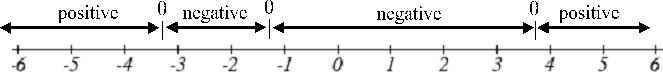
\includegraphics{images/image068.png}
\caption{}
\end{figure}

From our test values, we can determine this function is positive when
\textbackslash{}(x \textbackslash{}lt -3 \textbackslash{}) or
\textbackslash{}(x \textbackslash{}gt 4\textbackslash{}), or in interval
notation, \textbackslash{}( (-\textbackslash{}infty,-3)
\textbackslash{}cup (4,\textbackslash{}infty) \textbackslash{}).

To view this video please enable JavaScript, and consider upgrading to a
web browser that \href{http://videojs.com/html5-video-support/}{supports
HTML5 video}

\hypertarget{rational-functions}{%
\subsection{Rational Functions}\label{rational-functions}}

Rational functions are the ratios, or fractions, of polynomials. They
can arise from both simple and complex situations.

\hypertarget{example-5}{%
\paragraph{Example 5}\label{example-5}}

You plan to drive 100 miles. Find a formula for the time the trip will
take as a function of the speed you drive.

You may recall that multiplying speed by time will give you distance. If
we let \textbackslash{}(t\textbackslash{}) represent the drive time in
hours, and \textbackslash{}(v\textbackslash{}) represent the velocity
(speed or rate) at which we drive, then
\textbackslash{}(vt=\textbackslash{})distance. Since our distance is
fixed at 100 miles, \textbackslash{}(vt=100\textbackslash{}). Solving
this relationship for the time gives us the function we desired:
\textbackslash{}{[}t(v)=\textbackslash{}frac\{100\}\{v\}\textbackslash{}{]}

Notice that this is a transformation of the reciprocal toolkit function,
\textbackslash{}( f(x)=\textbackslash{}dfrac\{1\}\{x\}
\textbackslash{}). Several natural phenomena, such as gravitational
force and volume of sound, behave in a manner \textbf{inversely
proportional to the square} of another quantity. For example, the
volume, \textbackslash{}(V\textbackslash{}), of a sound heard at a
distance \textbackslash{}(d\textbackslash{}) from the source would be
related by \textbackslash{}( V=\textbackslash{}dfrac\{k\}\{d\^{}2\}
\textbackslash{}) for some constant value
\textbackslash{}(k\textbackslash{}). These functions are transformations
of the reciprocal squared toolkit function \textbackslash{}(
f(x)=\textbackslash{}dfrac\{1\}\{x\^{}2\} \textbackslash{}).

We have seen the graphs of the basic reciprocal function and the squared
reciprocal function from our review of toolkit functions. These graphs
have several important features.

\begin{figure}
\centering
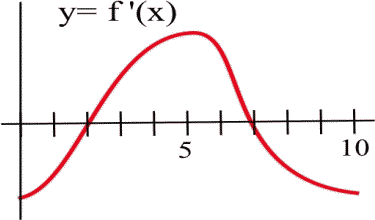
\includegraphics{images/image070.png}
\caption{\textbackslash{}( f(x)=\textbackslash{}frac\{1\}\{x\}
\textbackslash{})}
\end{figure}

\begin{figure}
\centering
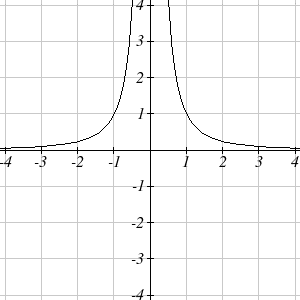
\includegraphics{images/image069.png}
\caption{\textbackslash{}( f(x)=\textbackslash{}frac\{1\}\{x\^{}2\}
\textbackslash{})}
\end{figure}

Let's begin by looking at the reciprocal function, \textbackslash{}(
f(x)=\textbackslash{}dfrac\{1\}\{x\} \textbackslash{}). As you well
know, dividing by zero is not allowed and therefore zero is not in the
domain, and so the function is undefined at an input of zero.

\hypertarget{short-run-behavior}{%
\subsubsection{Short Run behavior:}\label{short-run-behavior}}

As the input values approach zero from the left side (taking on very
small, negative values), the function values become very large in the
negative direction (in other words, they approach negative infinity). We
write: \textbackslash{}( x\textbackslash{}to 0\^{}- \textbackslash{}),
\textbackslash{}( f(x)\textbackslash{}to -\textbackslash{}infty
\textbackslash{}).

As we approach zero from the right side (small, positive input values),
the function values become very large in the positive direction
(approaching infinity). We write: as \textbackslash{}(
x\textbackslash{}to 0\^{}+ \textbackslash{}), \textbackslash{}(
f(x)\textbackslash{}to \textbackslash{}infty \textbackslash{}).

This behavior creates a \textbf{vertical asymptote}. An asymptote is a
line that the graph approaches. In this case the graph is approaching
the vertical line \textbackslash{}(x = 0\textbackslash{}) as the input
becomes close to zero.

\hypertarget{long-run-behavior}{%
\subsubsection{Long Run behavior:}\label{long-run-behavior}}

As the values of x approach infinity, the function values approach 0.
Also, as the values of x approach negative infinity, the function values
approach 0. Symbolically: as \textbackslash{}(
x\textbackslash{}to\textbackslash{}pm\textbackslash{}infty
\textbackslash{}), \textbackslash{}( f(x)\textbackslash{}to 0
\textbackslash{}).

Based on this long run behavior and the graph we can see that the
function approaches 0 but never actually reaches 0, it just "levels off"
as the inputs become large. This behavior creates a \textbf{horizontal
asymptote}. In this case the graph is approaching the horizontal line
\textbackslash{}( f(x)=0 \textbackslash{}) as the input becomes very
large in the negative and positive directions.

\hypertarget{vertical-and-horizontal-asymptotes}{%
\paragraph{Vertical and Horizontal
Asymptotes}\label{vertical-and-horizontal-asymptotes}}

A \textbf{vertical asymptote} of a graph is a vertical line
\textbackslash{}(x = a\textbackslash{}) where the graph tends towards
positive or negative infinity as the inputs approach
\textbackslash{}(a\textbackslash{}). As \textbackslash{}(
x\textbackslash{}to a \textbackslash{}), \textbackslash{}(
f(x)\textbackslash{}to\textbackslash{}pm\textbackslash{}infty
\textbackslash{}).

A \textbf{horizontal asymptote} of a graph is a horizontal line
\textbackslash{}( y=b \textbackslash{}) where the graph approaches the
line as the inputs get large. As \textbackslash{}(
x\textbackslash{}to\textbackslash{}pm\textbackslash{}infty
\textbackslash{}), \textbackslash{}( f(x)\textbackslash{}to b
\textbackslash{}).

\hypertarget{example-6}{%
\paragraph{Example 6}\label{example-6}}

Sketch a graph of the reciprocal function shifted two units to the left
and up three units. Identify the horizontal and vertical asymptotes of
the graph, if any.

Transforming the graph left 2 and up 3 would result in the function
\textbackslash{}( f(x)=\textbackslash{}dfrac\{1\}\{x+2\}+3
\textbackslash{}), or equivalently, by giving the terms a common
denominator,
\textbackslash{}{[}f(x)=\textbackslash{}dfrac\{3x+7\}\{x+2\}.\textbackslash{}{]}

Shifting the toolkit function would give us this graph. Notice that this
equation is undefined at \textbackslash{}(x = -2\textbackslash{}), and
the graph also is showing a vertical asymptote at \textbackslash{}(x =
-2\textbackslash{}). As \textbackslash{}( x\textbackslash{}to -2\^{}-
\textbackslash{}), \textbackslash{}( f(x)\textbackslash{}to
-\textbackslash{}infty \textbackslash{}), and as \textbackslash{}(
x\textbackslash{}to -2\^{}+ \textbackslash{}), \textbackslash{}(
f(x)\textbackslash{}to \textbackslash{}infty \textbackslash{}).

\begin{figure}
\centering
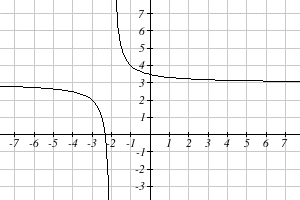
\includegraphics{images/image071.png}
\caption{}
\end{figure}

As the inputs grow large, the graph appears to be leveling off at output
values of 3, indicating a horizontal asymptote at \textbackslash{}(
y=3\textbackslash{}). As \textbackslash{}(
x\textbackslash{}to\textbackslash{}pm\textbackslash{}infty
\textbackslash{}), \textbackslash{}( f(x)\textbackslash{}to 3
\textbackslash{})

Notice that horizontal and vertical asymptotes get shifted left 2 and up
3 along with the function.

A general rational function is the ratio of any two polynomials.

\hypertarget{rational-function}{%
\paragraph{Rational Function}\label{rational-function}}

A \textbf{rational function} is a function that can be written as the
ratio of two polynomials, \textbackslash{}(P(x)\textbackslash{}) and
\textbackslash{}(Q(x)\textbackslash{}).
\textbackslash{}{[}f(x)=\textbackslash{}frac\{P(x)\}\{Q(x)\}=\textbackslash{}frac\{a\_0+a\_1
x+a\_2 x\^{}2+\textbackslash{}dots+a\_p x\^{}p\}\{b\_0+b\_1 x+b\_2
x\^{}2+\textbackslash{}dots+b\_q x\^{}q\}\textbackslash{}{]}

Rational functions can arise from real situations.

\hypertarget{example-7}{%
\paragraph{Example 7}\label{example-7}}

A large mixing tank currently contains 100 gallons of water, into which
5 pounds of sugar have been mixed. A tap will open pouring 10 gallons
per minute of water into the tank at the same time sugar is poured into
the tank at a rate of 1 pound per minute. Find the concentration (pounds
per gallon) of sugar in the tank after
\textbackslash{}(t\textbackslash{}) minutes.

Notice that the amount of water in the tank is changing linearly, as is
the amount of sugar in the tank. We can write an equation independently
for each:\textbackslash{}{[}\textbackslash{}text\{water\}=100+10t
\textbackslash{}qquad
\textbackslash{}text\{sugar\}=5+1t\textbackslash{}{]}

The concentration, \textbackslash{}(C\textbackslash{}), will be the
ratio of pounds of sugar to gallons of water:
\textbackslash{}{[}C(t)=\textbackslash{}frac\{5+t\}\{100+10t\}\textbackslash{}{]}

\hypertarget{vertical-asymptotes-of-rational-functions}{%
\paragraph{Vertical Asymptotes of Rational
Functions}\label{vertical-asymptotes-of-rational-functions}}

The \textbf{vertical asymptotes} of a rational function will occur where
the denominator of the function is equal to zero and the numerator is
not zero.

\hypertarget{horizontal-asymptote-of-rational-functions}{%
\paragraph{Horizontal Asymptote of Rational
Functions}\label{horizontal-asymptote-of-rational-functions}}

The \textbf{horizontal asymptote} of a rational function can be
determined by looking at the degrees of the numerator and denominator.

\begin{itemize}
\tightlist
\item
  Degree of denominator \textgreater{} degree of numerator: Horizontal
  asymptote at \textbackslash{}( y=0 \textbackslash{}).
\item
  Degree of denominator \textless{} degree of numerator: No horizontal
  asymptote.
\item
  Degree of denominator = degree of numerator: Horizontal asymptote at
  ratio of leading coefficients, \textbackslash{}(
  y=\textbackslash{}dfrac\{a\_p\}\{b\_q\} \textbackslash{})
  (\textbackslash{}(p\textbackslash{}) and
  \textbackslash{}(q\textbackslash{}) are equal in this case).
\end{itemize}

\hypertarget{example-8}{%
\paragraph{Example 8}\label{example-8}}

In the sugar concentration problem from earlier, we created the equation
\textbackslash{}( C(t)=\textbackslash{}frac\{5+t\}\{100+10t\}
\textbackslash{}). Find the horizontal asymptote and interpret it in
context of the scenario.

Both the numerator and denominator are linear (degree 1), so since the
degrees are equal, there will be a horizontal asymptote at the ratio of
the leading coefficients. In the numerator, the leading term is t, with
coefficient 1. In the denominator, the leading term is
\textbackslash{}(10t\textbackslash{}), with coefficient 10. The
horizontal asymptote will be at the ratio of these values: As
\textbackslash{}( t \textbackslash{}to \textbackslash{}infty
\textbackslash{}), \textbackslash{}( C(t)\textbackslash{}to
\textbackslash{}frac\{1\}\{10\} \textbackslash{}). This function will
have a horizontal asymptote at \textbackslash{}(
y=\textbackslash{}frac\{1\}\{10\} \textbackslash{}).

This tells us that as the input gets large, the output values will
approach \textbackslash{}( \textbackslash{}frac\{1\}\{10\}
\textbackslash{}). In context, this means that as more time goes by, the
concentration of sugar in the tank will approach one tenth of a pound of
sugar per gallon of water or \textbackslash{}(
\textbackslash{}frac\{1\}\{10\} \textbackslash{}) pounds per gallon.

\hypertarget{example-9}{%
\paragraph{Example 9}\label{example-9}}

Find the horizontal and vertical asymptotes of the function
\textbackslash{}{[}f(x)=\textbackslash{}frac\{(x-2)(x+3)\}\{(x-1)(x+2)(x-5)\}.\textbackslash{}{]}

First, note this function has no inputs that make both the numerator and
denominator zero, so there are no potential holes. The function will
have vertical asymptotes when the denominator is zero, causing the
function to be undefined. The denominator will be zero at
\textbackslash{}(x =\textbackslash{}) 1, -2, and 5, indicating vertical
asymptotes at these values.

The numerator has degree 2, while the denominator has degree 3. Since
the degree of the denominator is greater than the degree of the
numerator, the denominator will grow faster than the numerator, causing
the outputs to tend towards zero as the inputs get large, and so as
\textbackslash{}(
x\textbackslash{}to\textbackslash{}pm\textbackslash{}infty
\textbackslash{}), \textbackslash{}( f(x)\textbackslash{}to 0
\textbackslash{}). This function will have a horizontal asymptote at
\textbackslash{}( y=0 \textbackslash{}).

As with all functions, a rational function will have a vertical
intercept when the input is zero, if the function is defined at zero. It
is possible for a rational function to not have a vertical intercept if
the function is undefined at zero.

Likewise, a rational function will have horizontal intercepts at the
inputs that cause the output to be zero (unless that input corresponds
to a hole). It is possible there are no horizontal intercepts. Since a
fraction is only equal to zero when the numerator is zero, horizontal
intercepts will occur when the numerator of the rational function is
equal to zero.

To view this video please enable JavaScript, and consider upgrading to a
web browser that \href{http://videojs.com/html5-video-support/}{supports
HTML5 video}

\hypertarget{example-10}{%
\paragraph{Example 10}\label{example-10}}

Find the intercepts of
\textbackslash{}{[}f(x)=\textbackslash{}frac\{(x-2)(x+3)\}\{(x-1)(x+2)(x-5)\}.\textbackslash{}{]}

We can find the vertical intercept by evaluating the function at zero:
\textbackslash{}{[}f(0)=\textbackslash{}frac\{(0-2)(0+3)\}\{(0-1)(0+2)(0-5)\}=\textbackslash{}frac\{-6\}\{10\}=-\textbackslash{}frac\{3\}\{5\}.\textbackslash{}{]}

The horizontal intercepts will occur when the function is equal to zero:
\textbackslash{}{[} \textbackslash{}begin\{align*\} 0=\&
\textbackslash{}frac\{(x-2)(x+3)\}\{(x-1)(x+2)(x-5)\}
\textbackslash{}qquad \textbackslash{}text\{(This is zero when the
numerator is zero.)\}\textbackslash{}\textbackslash{} 0=\&
(x-2)(x+3)\textbackslash{}\textbackslash{} x=\& 2, -3.
\textbackslash{}end\{align*\} \textbackslash{}{]}

\begin{longtable}[]{@{}ll@{}}
\toprule
\endhead
\href{section1-5.php}{← Previous Section} & \href{section1-7.php}{Next
Section →}\tabularnewline
\bottomrule
\end{longtable}
